\documentclass[12pt]{article}
\usepackage{xcolor}
  \definecolor{yb-blue}{rgb}{0,0.5765,0.8196}
\usepackage{hyperref}
  \hypersetup{colorlinks=true,urlcolor=yb-blue,pdfborder={0 0 0}}
\usepackage{mathpazo}
\usepackage{graphicx}
\usepackage[absolute]{textpos}
  \TPGrid{16}{16}
\usepackage[top=2\TPVertModule, bottom=2\TPVertModule, left=3\TPHorizModule, right=2\TPHorizModule]{geometry}
\usepackage{tikz}
\usepackage{fancyhdr}
  \pagestyle{fancy}
  \renewcommand{\headrulewidth}{0pt}
  \fancyhf{}
  \rhead{
    \begin{textblock}{1}[0,0](0,0){
      \tikz[x=\TPHorizModule,y=\TPVertModule] \filldraw[fill=yb-blue, draw=none] (0,0) rectangle (2,16);
    }\end{textblock}
  }

\begin{document}
\setlength{\topskip}{0mm}
\setlength{\parindent}{0pt}
\setlength{\parskip}{6pt}
\raggedright
\large
\interfootnotelinepenalty=10000

\begin{textblock}{2.4}[1,0](14,2){
  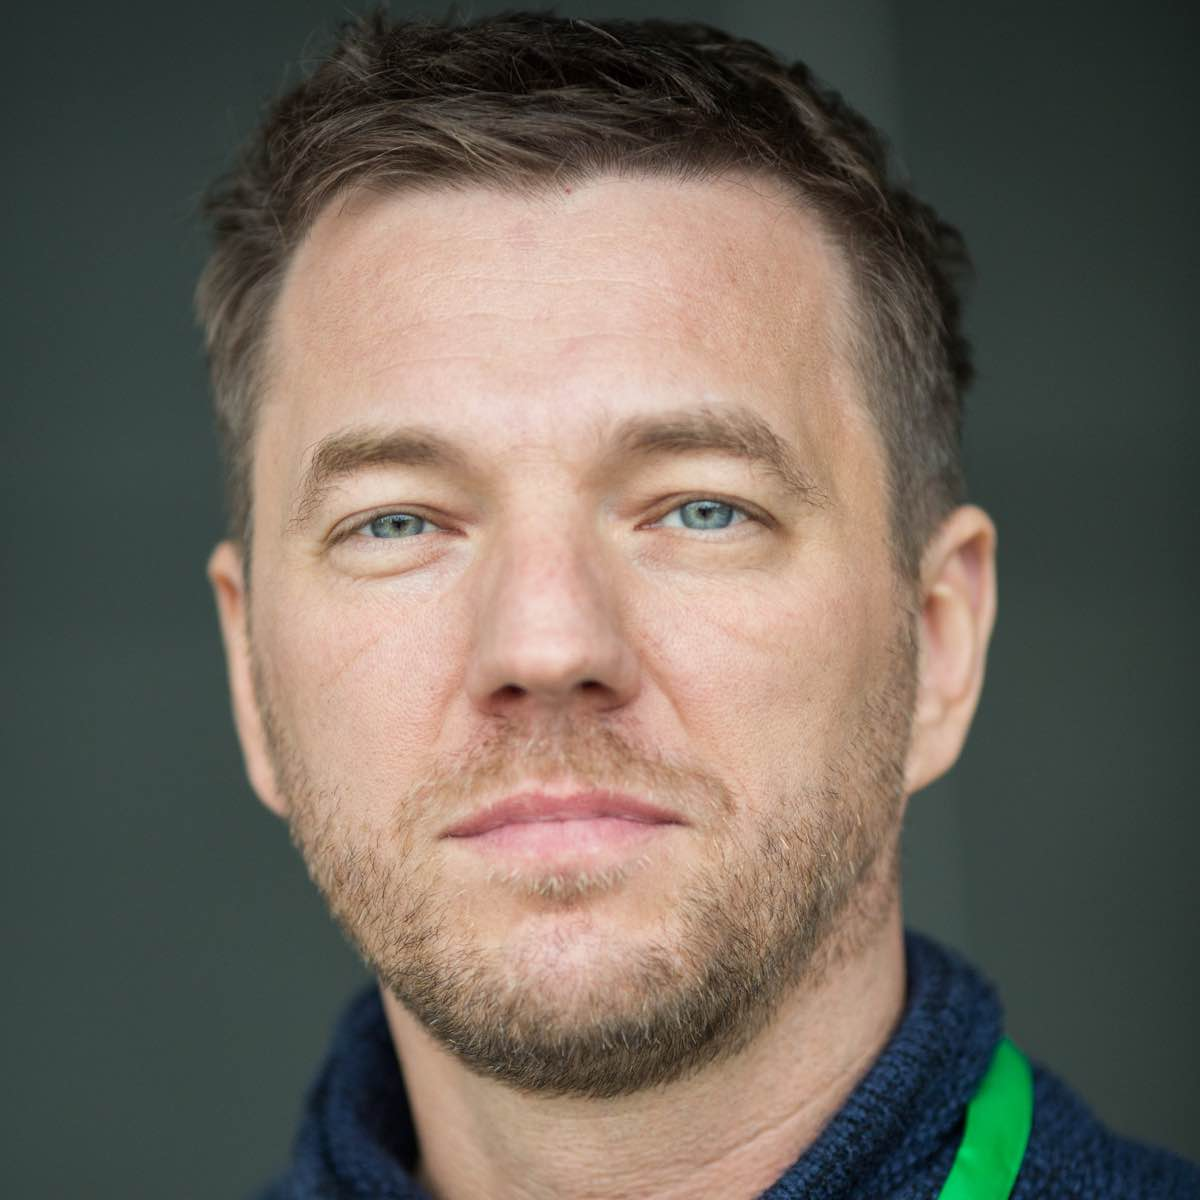
\includegraphics[width=\textwidth]{../images/face-1200x1200.jpg}
}\end{textblock}

\textbf{\Large Yeg\'or Bugay\'enko}\\%
\href{mailto:yegor256@gmail.com}{yegor256@gmail.com}\\
%
(408) 692-4742

\vspace{1em}

Founder and CEO of \textbf{\href{https://www.zerocracy.com}{Zerocracy}} since 2016.

Inventor of eXtremely Distributed Software Development (\href{http://www.xdsd.org}{XDSD}).

Managing software projects since 1998 (in seven companies).

Author of \textbf{\href{http://www.yegor256.com/elegant-objects.html}{Elegant Objects}},
  an OOP book series.

Regular \textbf{blogger} at \href{http://www.yegor256.com/}{yegor256.com} since 2014.

Proud holder of \textbf{SCEA} and
  \textbf{PMP} certifications.

Creator of \href{http://www.takes.org}{Takes},
  \href{http://www.cactoos.org}{Cactoos},
  \href{http://www.jcabi.com}{JCabi},
  \href{http://www.rultor.com}{Rultor},
  \href{http://www.qulice.com}{Qulice} and
  \href{http://www.yegor256.com/pets.html}{others}.

\textbf{M.Sc.} in Computer Science,
  \href{https://en.wikipedia.org/wiki/Oles_Honchar_Dnipro_National_University}{graduated} in 1998.

Regular \textbf{\href{http://www.yegor256.com/talks.html}{speaker}}
  at software conferences, incl. JPoint, GeeCON, AgileDays, {\O}redev, GeekOUT, NDC, JEEConf.

Full member of ACM and IEEE since 1996.

Hands-on Java/C++/Ruby programmer
  (1.7K+ \textbf{\href{https://github.com/yegor256}{GitHub}} followers).

Regular contributor to \textbf{StackOverflow}
  (check my \href{https://stackexchange.com/users/63162/yegor256}{60K+ profile}).

Named author on a few patent applications
  (e.g. \href{https://www.google.com/patents/US20120023476}{12/840,306}).

Author of a few academic CS \textbf{publications}
  (e.g. \href{link.springer.com/chapter/10.1007/978-3-642-02152-7_6}{this}).

Member of \href{http://standards.ieee.org/develop/wg/730.html}{IEEE 730 committee}.

Fond of tennis, kyokushin karate, snow boarding and surfing.

Fond of \href{http://www.yegor256.com/paintings.html}{art} (painting).

Active on
  \href{https://twitter.com/intent/follow?screen_name=yegor256}{Twitter} (15K followers),
  \href{https://www.facebook.com/yegor256}{Facebook} (2K),
  and \href{https://instagram.com/yegor256}{Instagram} (6K).

\end{document}
